\documentclass{article}

% \usepackage[letterpaper, margin=2cm]{geometry}
% \usepackage{amsmath,graphicx}
% \usepackage{multicol}
% \usepackage[font=scriptsize,labelfont=bf]{caption}
% \usepackage{sectsty}
% \usepackage{booktabs}

\usepackage{amsmath,graphicx}
\usepackage{sectsty}
\usepackage[letterpaper, margin=2.0cm]{geometry}
\usepackage{amsmath,graphicx}
\usepackage{multicol}
\usepackage{array}
\usepackage{csvsimple}
\usepackage{booktabs}
\usepackage{multirow}
\usepackage{float}
\usepackage{array}
\usepackage[font=scriptsize,labelfont=bf]{caption}
\usepackage{booktabs}

\usepackage{biblatex}


\addbibresource{refs.bib}
\sectionfont{\fontsize{12}{15}\selectfont}
\captionsetup{width=\textwidth}
\graphicspath{./}

\title{Hydroelectric Turbine PID Speed Governor}
\author{
    Anderson, Colin
    \and
    Potter, Kalen
    \and
    Tsosie, Naakaii
    \and
    VanShaar, Janson
}
\date{}


\begin{document}
    \maketitle

    \thispagestyle{plain}
    
    \noindent\makebox[\linewidth]{\rule{\textwidth}{0.4pt}}

    \begin{center}
        \textbf{Abstract}
    \end{center}


    A project exploring the real scenario of the Sayano-Shushenskaya power station accident that occurred in 2009.  A simulated model of a single power generation system at the site is developed. The model shows how the opening of the water flow gate is changed through a typical year to reach maximum power generation without damaging the turbine.  The model is then fitted with a First Order Plus Dead Time (FOPDT) model to generate controller parameters for a PID controller that automates the opening and closing of the watergate.  Implications, environmental factors, and public safety of using the system are also discussed.

    \noindent\makebox[\linewidth]{\rule{\textwidth}{0.4pt}}

    \begin{multicols*}{2}
        \newlength{\mywidth}
        \setlength{\mywidth}{\linewidth}
        \addtolength{\mywidth}{-0.5\columnsep}

        \section{Introduction}

        On 17 August 2009, the Sayano-Shushenskaya hydro-electric power station in Russia failed catastrophically.  The cause of failure was determined to be from operating the power station under conditions that caused excess vibrations \cite{SayanoAccidentUpdate}. These vibrations fatigued the system, eventually causing the turbines to explode and damage the surrounding structures. The accident killed 75 people, caused widespread power outages, and cost approximately 41 billion rubles (1.25 billion USD) \cite{sayanoDam}.
        
        \section{Objective}

        The turbines in the plant were rated for safe operation between the bands of 0-350 MW and 550-650 MW \cite{sayWiki}. Our objective is to design a PID controller to control the power output.  The process variable will be power output and the controller output will be inlet gate opening.

        \section{Theory}

        We are modeling a turbine power generation system, with a desire to maintain the power output within certain “safety zones” in order to reduce vibrations on the generator. We control the power output of the system by adjusting the dam gate valve in order to let water flow through. Thus, the input for the power generation model is the gate height, and the output is the power produced by the turbine. These two variables are related through a series of equations. The first is: 

        \begin{equation}\label{flowEq}
            q = A \sqrt{2gh}
        \end{equation}

        $q$ is the volumetric flow rate, $h$ is the height of the water in relation to the turbine entrance, and $A$ is the area of the gate that is available for water to flow through. In this situation, $h$ is a variable because the dam level will change seasonally throughout the year, and $A$ will be change with the height of the gate (controller output). We then plug Equation \ref{flowEq} into our overall energy balance to generate our physics based model (Equation \ref{powerEq}).

        \begin{equation}\label{powerEq}
            W=\eta \rho gA\sqrt{2gh}\Delta z
        \end{equation}

        $W$ is the turbine power output, $\eta$ is the turbine efficiency (which is a constant at $0.8286$), $\Delta z$ is the height of the gate, and $\rho$ is the density of water (assumed to be constant at $998.29\ kg/m^3$). Our process will be automatically adjusting the gate height to account for the dam level, in order to keep the power output within acceptable ranges.

        Further theory, beyond the scope of this report, can be found from the following sources: “2009 accident update” \cite{SayanoAccidentUpdate} gives a detailed look at the background of the 2009 accident, “Hydro-turbine governor control: theory, techniques and limitations” \cite{htgc} outlines PID controller theory used in power plants.

        \section{Data Simulation}

        Due to the nature of the subject, we opted for simulated data and responses. To design a PID control system, some starting parameters must be derived using an FOPDT model. The turbine has two zones of operation, a low-power zone and a high-power zone. If the gate height is treated as the controller input then the controller gain is not the same for each zone. Our solution was to use power output as the controller input, treat dam level as a disturbance variable, and have the gate height be the controller output.

        \vspace{1ex}

        \begin{minipage}{0.9\columnwidth}
            \captionof{table}{FOPDT Parameters}\label{foParams}
            \vspace{-1ex}
            \begin{center}
            \begin{tabular}{cccc}
                    \toprule
                    $K_p$ & $K_d$ & $\tau_p$ & $\theta_p$ \\
                    \midrule
                    1.0 & 0.0 & 1.8 days & 0.0 days
                \end{tabular}
            \end{center}
        \end{minipage}

        Equation \ref{powerEq} was used to generate an open-loop response to a change in dam height (Figure \ref{fopdt}). This was used to generate the FOPDT parameters in Table \ref{foParams}.
        
        \vspace{5mm}
        \noindent
        \begin{minipage}{0.49\textwidth}
            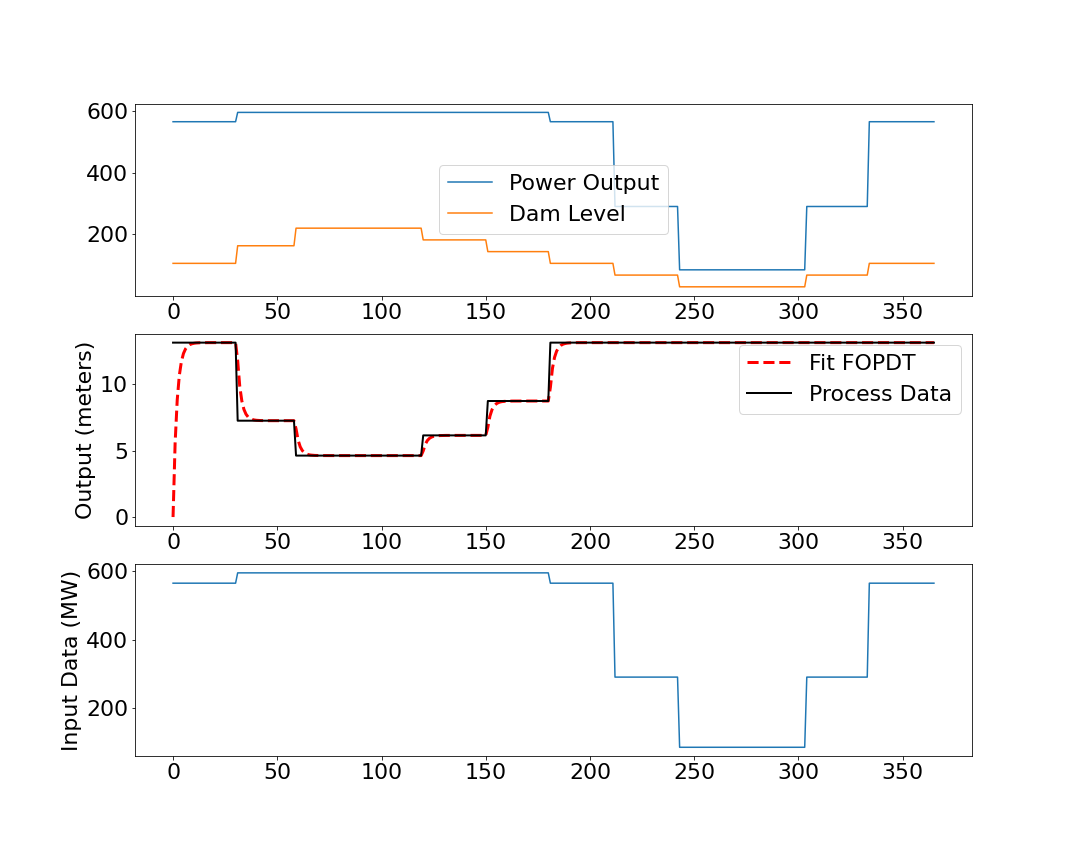
\includegraphics[width=\textwidth]{FOPDT_big.png}
            \captionof{figure}{FOPDT Model Fit}\label{fopdt}
        \end{minipage}
            
        \section{PID Controller}
    
        The parameters in Table \ref{foParams} can be used to begin tuning the PID controller.  During the tuning process, we had to reduce $K_p$ by 25\%, because of oscillations that occurred and caused the system to occasionally spend excess time outside the safety zone. The final tuning parameters are in Table \ref{pidParams}. The performance of the untuned controller is demonstrated in Figure \ref{untunedCon} and the tuned controller in Figure \ref{tunedCon}.

        \begin{minipage}{0.9\columnwidth}
            \captionof{table}{PID Parameters}\label{pidParams}
            \vspace{-1ex}
            \begin{center}
            \begin{tabular}{ccc}
                    \toprule
                    $K_c$ & $\tau_I$ & $\tau_D$ \\
                    \midrule
                     1.8 & 1.8 days & 0.0 days
                \end{tabular}
            \end{center}
        \end{minipage}

        Occasionally the systems need to be serviced and turned off.  Due to the limitations of the controller, initial startup of the system and changing from high to low power will require manual adjustment; otherwise the system will be operating outside the safety zones for a whole week, where it can be damaged severely.  Once the adjustments are made, then the controller can be reactivated for safe automated operation.

        \vspace{5mm}
        \noindent
        \begin{minipage}{0.49\textwidth}
            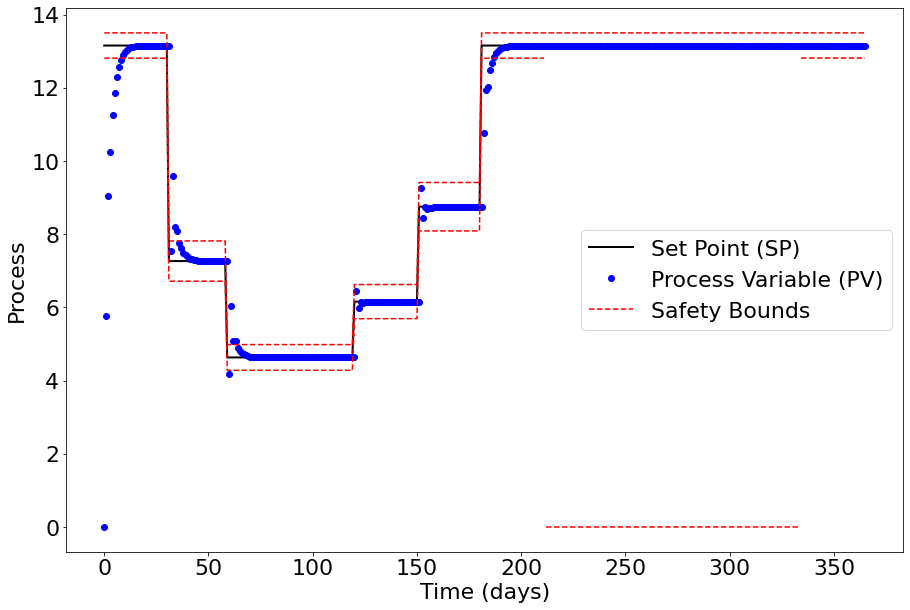
\includegraphics[width=\textwidth]{projectPID_untuned.png}
            \captionof{figure}{Untuned PID Controller}\label{untunedCon}
        \end{minipage}

        \noindent
        \begin{minipage}{0.49\textwidth}
            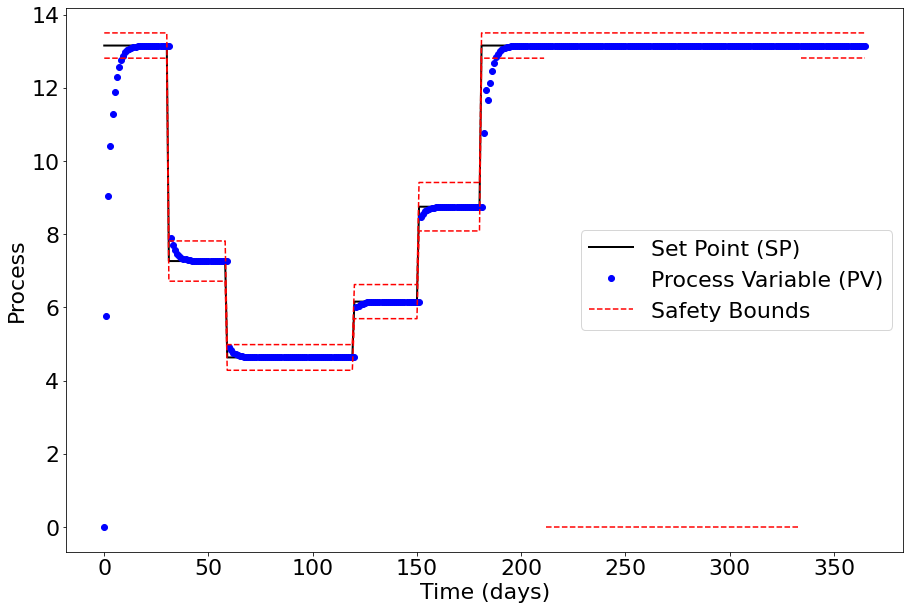
\includegraphics[width=\textwidth]{projectPID_tuned.png}
            \captionof{figure}{Tuned PID Controller}\label{tunedCon}
        \end{minipage}

        \section{Conclusion}
        
        In conclusion, we were able to design and code a PID controller to manage the valve that controls the input flow.  One major assumption made was that the properties of the water are constant.  Another assumption is that all work generated from the dam comes from potential energy.  A further study would need to be done to find the pressure drops and work along the gate head that would be lost, as well as develop a higher order model that would account for the gain changes that were mentioned. This is a simple start to designing and coding a fully automated system for the hydroelectric station.  Though this would not be the best to implement into a current system, it does model a basic outline of the dam PID controller.
        
    \end{multicols*}

        \pagebreak
        
        \begin{multicols*}{2}
            
            \section{Non-Technical Considerations}
            
            Turbine speed governors are a critical part of a hydroelectric power plant, and failure has catastrophic consequences. The 2009 accident at the Sayano-Shushenskaya power plant killed 75 people and led to widespread power outages. Therefore, it is important to not only consider the impact of the control system, but the impact of the dam and hydroelectric power plant.
            
            The construction of a dam is a massive project that has consequences for those living in the area. Changes to water flow and the creation of a reservoir can negatively impact local wildlife as well as displace local residents; such was the case with the construction of Bhakra Dam in northern India. 
            
            The generation of electricity impacts many aspects of life, including public welfare and the environment. The purpose of a hydraulic dam is to generate clean energy which protects the environment. Access to that energy provides people with a higher quality of life and greater economic opportunity.
            
            This research would also include emergency preparations in case the dam breaks and overflow preparations. Along with this research, cities that would be impacted by an accident at the dam would need to create emergency plans.
            
            When designing the turbine, to reduce environmental stress, we recommend using a filter before the entrance of the dam, so that aquatic life and debris do not enter the turbine. We also recommend doing research into the effects of the dam on wildlife and the heights of streams in surrounding areas. Emergency plans need to be created to account for if these filters fail. These filters also need to be cleaned and replaced often.
            There are many benefits that a hydroelectric power plant provides, and a good control system ensures that the plant remains operational.
            
        \end{multicols*}
            
            
    \pagebreak
    \nocite{*}
    \printbibliography
\end{document}